\section{Design Factor}\label{sec:DF}

The Design Factor (\(N_u\)/\(N_y\)) is used to obtain an ``allowable'' or ``working'' stress for design calculations. The design factor may be based on a number of failure modes, such as \ac{UTS} or endurance limit.

When considering the \ac{UTS}, the Design Factor (\(N_u\)) is:

\begin{equation}
    N_u = a.b.c.d.k 
\end{equation}

And the allowable stress is calculated by:

\begin{equation}
    \text{Allowable Stress} = \frac{S_\text{UTS}}{N_u}
\end{equation}

When considering the \acf{YS}, the Design Factor (\(N_y\)) is:

\begin{equation}
    N_y = b.c.d.k
\end{equation}

And the allowable stress is calculated by:

\begin{equation}
    \text{Allowable Stress} = \frac{S_\text{y}}{N_y} 
\end{equation}

The five factors \(a\), \(b\), \(c\), \(d\) and \(k\) ensure that we consider the following in our calculations: 

\begin{description}
    \item[a] ratio between \ac{UTS} and \ac{YS} for your material
    \item[b] fatigue factor
    \item[c] shock factor
    \item[d] factor of safety (Pugsley's Method)
    \item[k] stress concentration factor
\end{description}

The\marginnote{a: UTS / YS ratio} ratio of the ultimate strength of the material to its yield strength (sometimes the elastic limit). If the yield strength is not known then this factor is used to estimate what it would be:

\begin{description}
    \item[\(a=2\)] for ductile material
    \item[\(a=1.5\)] for heat treated and tempered alloys
\end{description}

For cast iron, which has no real elastic limit, failure occurs suddenly at the ultimate tensile strength, and there is no sense in applying this factor at all.

The\marginnote{b: Fatigue Factor} fatigue factor can be calculated using the Goodman Criterion but in general and for the purpose of this exercise, you should consider two scenarios:

%used to quantify the interaction of mean and alternating stresses on the fatigue life of a material.

%\begin{equation}
%  \sigma_\text{a} = \sigma_\text{fat}\times\left(1-\frac{\sigma_\text{m}}{\sigma_\text{ts}}\right).
%\end{equation}

%\noindent Where $\sigma_\text{a}$ is the alternating stress, $\sigma_\text{m}$ is the mean stress, $\sigma_\text{fat}$ is the fatigue limit for completely reversed loading, and $\sigma_\text{ts}$ is the ultimate tensile strength of the material. But in general and for the purpose of this exercise, you should consider two scenarios:

\begin{description}
    \item[\(b=1\)] for a dead load, or a single-plane load varying between 0 and a maximum.
    \item[\(b=1.5\)] for a load that varies between tension and compression
\end{description}

The\marginnote{c: Shock Factor} dynamic forces imposed by shock loading can be many times the static loads that a shaft is designed towards. If there is potential for a shock load, a safety factor should be included to account. Again, you should consider two cases.

\begin{description}
    \item[\(c=1\)] when loads are gradually applied
    \item[\(c=2\)] when loads are suddenly applied
\end{description}

To investigate the shock loads in detail, analysis of the elongation and energy absorption capability of material and geometry would be required.

The\marginnote{d: ``Factor of Safety''} ``Factor of Safety'' or uncertainty factor can be considered the ``real'' safety factor. 

If all the other factors (a,b,c,k) are properly computer and accounted for, and the ``design factor'' made equal to their product, the design will still have nor margin of safety to allow for unexpected variation in load or material quality. It may be on the point of failure and these factors may be indeterminate, or extremely complex, or uncertain.

The factor d provide for these conditions, The value taken for d will be dependent on the judgement of the designer, but will include the consideration of the following:

\begin{enumerate}
    \item Degree of accuracy of stress computations \emph{(I.e.\ the reliance that can be placed on the estimation of and the assumptions made in calculating the stresses.)}
    \item Degree of reliability of the material \emph{I.e.\ the conformance to specification of the material chosen and the property chosen to represent the behaviour of the material under the specified loading.}
    \item Degree of uncertainty of loading \emph{I.e.\ How reliable the load specification is both in terms of magnitude, point of application, distribution of loading and inclusion of other loads such as handling, transportation etc.}
    \item Degree of reliability of specification \emph{I.e.\ How reliable the ``specification'' is in terms of defining the function etc.}
    \item Initial stresses \emph{I.e.\ Presence of residual stresses associated with manufacture, forming or assembly etc.}
    \item Reliability of manufacture \emph{I.e.\ Variability of heat treatments, surface finishes, dimensional tolerances etc.}
    \item Indeterminate or unexpected loads \emph{I.e.\ Errors in handling, changes in loading due to wear of critical parts etc.}
    \item Operating environment \emph{I.e.\ Ambient temperature (high or low), corrosion etc.}
    \item Consequences of failure \emph{I.e.\ Danger to life, ease of repair, cost of failure etc.}
\end{enumerate}

A safety factor may be defined by a Code of Practice, Company Policy, experience of designer. Codes of Practice specifying Safety Factors are often associated with specialised industries for products such as boilers, buildings etc. Companies dealing with specialised products frequently have their own specified factors of safety. Caution should be exercised where the design differs from the ``norm''. Experienced designers will often have developed their own safety factors for application to their design speciality.


In\marginnote{Calculating d using Pugsley's Method} 1966, Pugsley \mycite{howard1967} devised a general methodology for determining the safety factor, which takes the manufacturing, operational characteristics, and seriousness of failure into account\footnote{For more information on Safety Factors please see \cref{appendix-safety}}.

\begin{equation}
    d = X.Y
\end{equation}

\begin{description}
    \item[\(X\)] is chosen based on three factors related to manufacture and operation.
    \item[\(Y\)] is chosen based on seriousness of failure related to personnel and to economic impact.
\end{description}

To calculate the value of \(X\), one has to determine the quality of the component in three areas:

\begin{description}
    \item[A] Materials, workshop, inspection and manufacture
    \item[B] Loading and control over it
    \item[C] Quality of assessment of strength, analysis methods and accuracy
\end{description}

Each are scored as either Very Good (VG), Good (G), Fair (F) or Poor (P). Using these scores, the value for \(X\) can be calculated using \cref{tbl-pugsley-x}.

\begin{table}[h!]
  \caption{Calculating $X$}\label{tbl-pugsley-x}
  \center{}
  \begin{tabular}{l c | c c c c}
    \toprule
    & B = & VG & G & F & P \\
    A = & C = & & & & \\
    \midrule
    VG & VG & 1.1 & 1.3 & 1.5 & 1.7 \\
    VG & G & 1.2 & 1.45 & 1.7 & 1.95 \\
    VG & F & 1.3 & 1.6 & 1.9 & 2.2 \\
    VG & P & 1.4 & 1.75 & 2.1 & 2.45 \\
    \midrule
    G & VG & 1.4 & 1.55 & 1.8 & 2.05 \\
    G & G & 1.45 & 1.75 & 2.05 & 2.35 \\
    G & F & 1.6 & 1.95 & 2.3 & 2.65 \\
    G & P & 1.75 & 2.15 & 2.55 & 2.95 \\
    \midrule
    F & VG & 1.5 & 1.8 & 2.1 & 2.4 \\
    F & G & 1.7 & 2.05 & 2.4 & 2.75 \\
    F & F & 1.9 & 2.3 & 2.7 & 3.1 \\
    F & P & 2.1 & 2.55 & 3.00 & 3.45 \\
    \midrule
    P & VG & 1.7 & 2.15 & 2.4 & 2.75 \\
    P & G & 1.95 & 2.35 & 2.75 & 3.15 \\
    P & F & 2.2 & 2.65 & 3.1 & 3.55 \\
    P & P & 2.45 & 2.95 & 3.45 & 3.95 \\
    \bottomrule
  \end{tabular}
\end{table}

To calculate the value of \(Y\), one has to assess the potential impact of the failing with respect to two areas:

\begin{description}
  \item[D] Seriousness of danger to personnel
  \item[E] Seriousness of economic consequences
\end{description}

These are scores Not Serious, Serious and Very Serious. Table~\ref{tbl-pugsley-y} is then used to look-up the respective \(Y\) value.

\begin{table}
  \caption{Calculating $Y$}\label{tbl-pugsley-y}
  \center{}
  \begin{tabular}{c c c c}
    \toprule
    D = & Not Serious & Serious & Very Serious \\
    E = & & & \\
    \midrule
    Not Serious & 1 & 1.2 & 1.4 \\
    Serious & 1.1 & 1.3 & 1.5 \\
    Very Serious & 1.2 & 1.4 & 1.6 \\
    \bottomrule
  \end{tabular}
\end{table}

This\marginnote{k: Stress Concentration Factor} allows for the fact that there may be sudden changes in the geometry of a part. An example is fillets that provide places where localised stresses are higher than those determined by simple stress analysis. A wealth of empirical and analytical studies have been performed to determine the stress concentration factors for features, such as fillets and circlip grooves (\cref{fig-stress-fillet,fig-stress-circlip}, respectively). 

\begin{figure*}[t!]
  
    \hfill{}
    \subfloat[Bending]{
        \includestandalone[width=0.45\textwidth]{05_design_factor/fillet-bending}
        %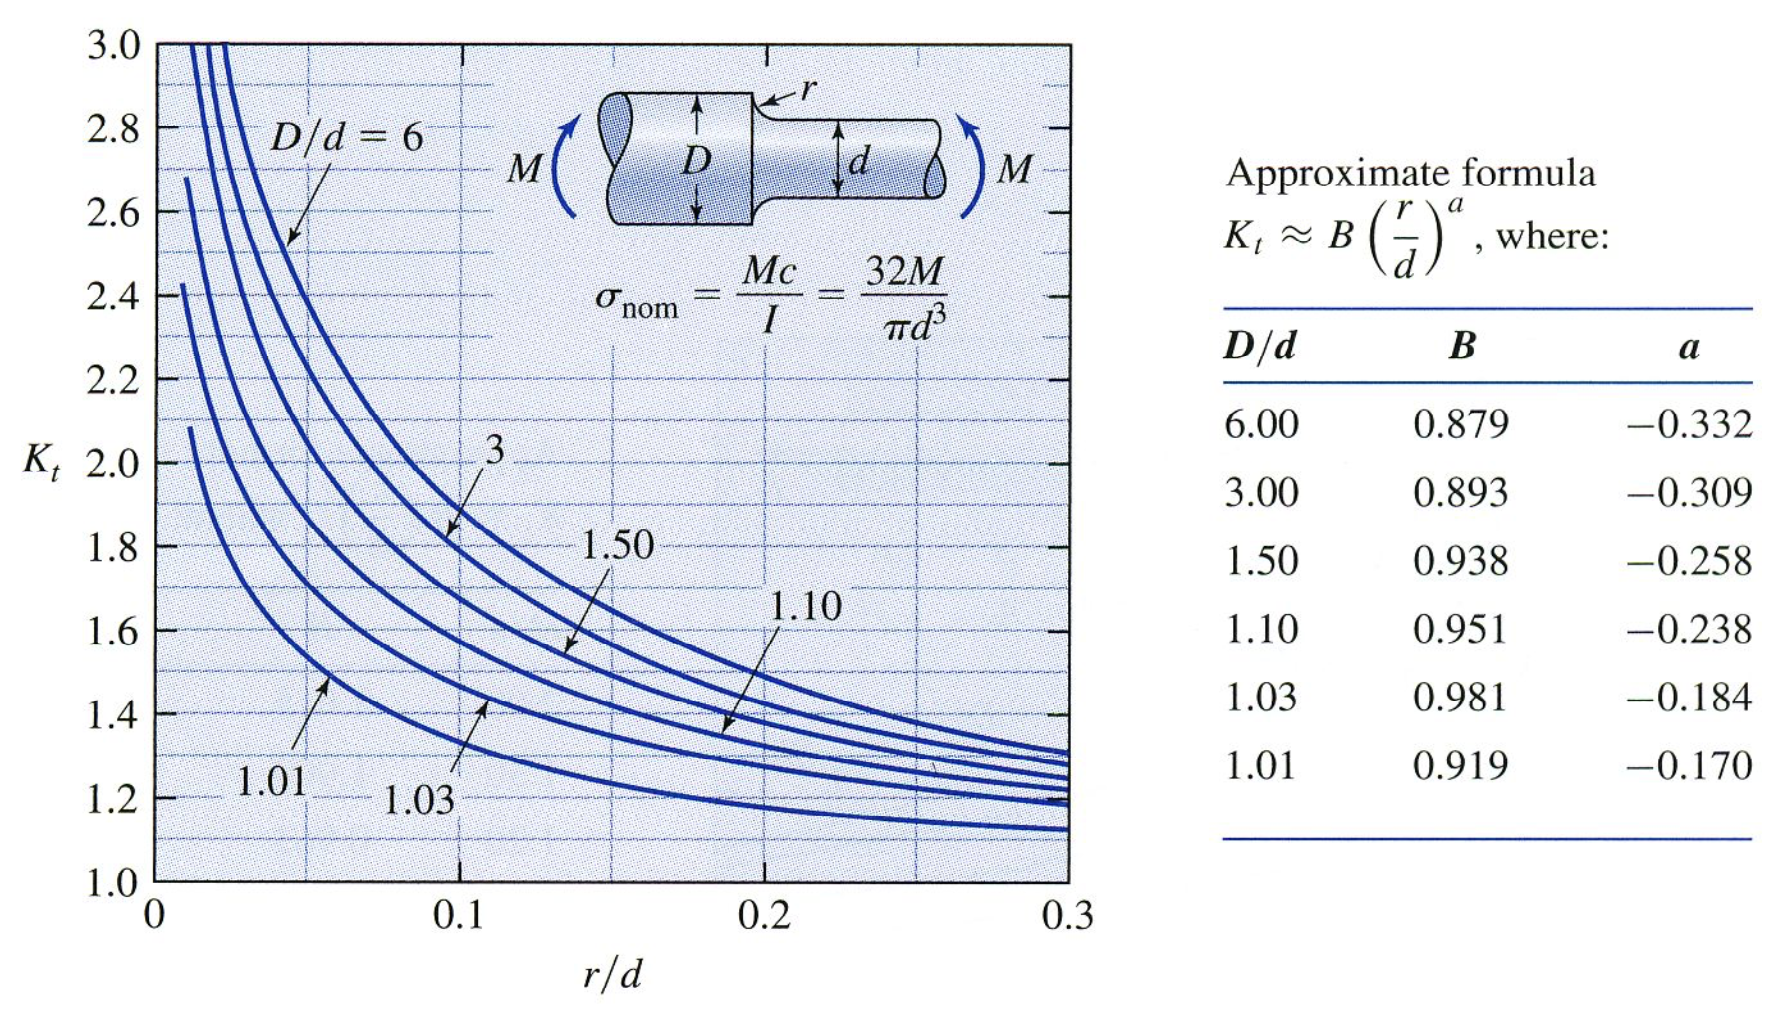
\includegraphics[width=0.45\textwidth]{05_design_factor/fillet-bending.png}
    }
    \hfill{}
    \subfloat[Torsion]{
        \includestandalone[width=0.45\textwidth]{05_design_factor/fillet-torsion}
        % 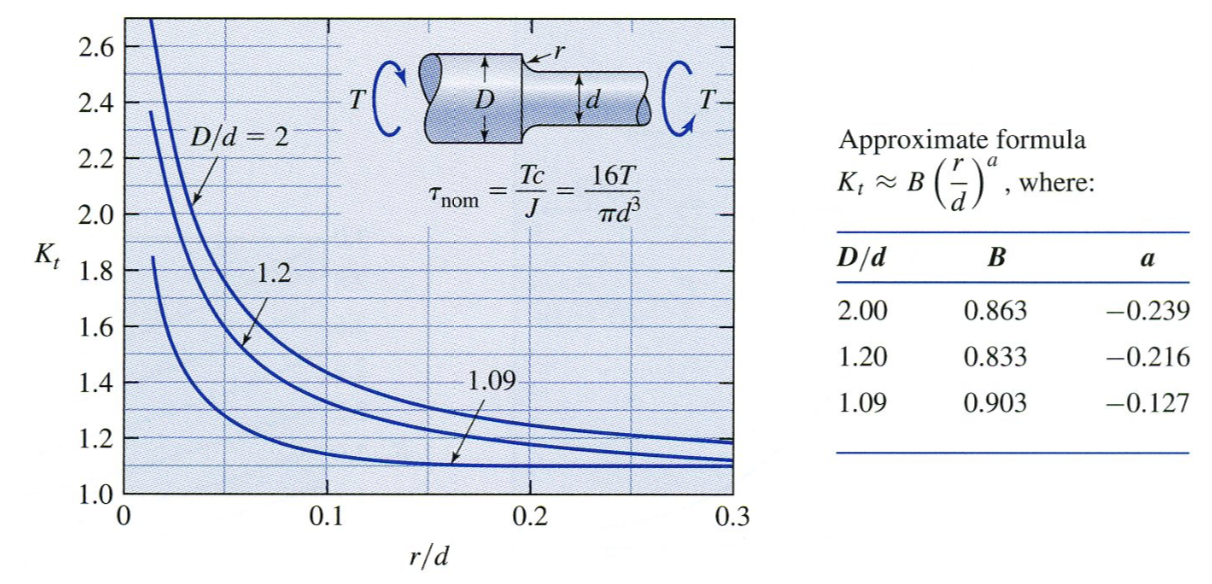
\includegraphics[width=0.45\textwidth]{05_design_factor/fillet-torsion.png}
    }
    \hfill{}
    
    \vspace{1em}
    \caption{Fillet stress concentration factors for shafts}\label{fig-stress-fillet}
\end{figure*}

\begin{figure*}[t]
    
    \hfill{}
    \subfloat[Bending]{
        \includestandalone[width=0.45\textwidth]{05_design_factor/circlip-groove-bending}
        %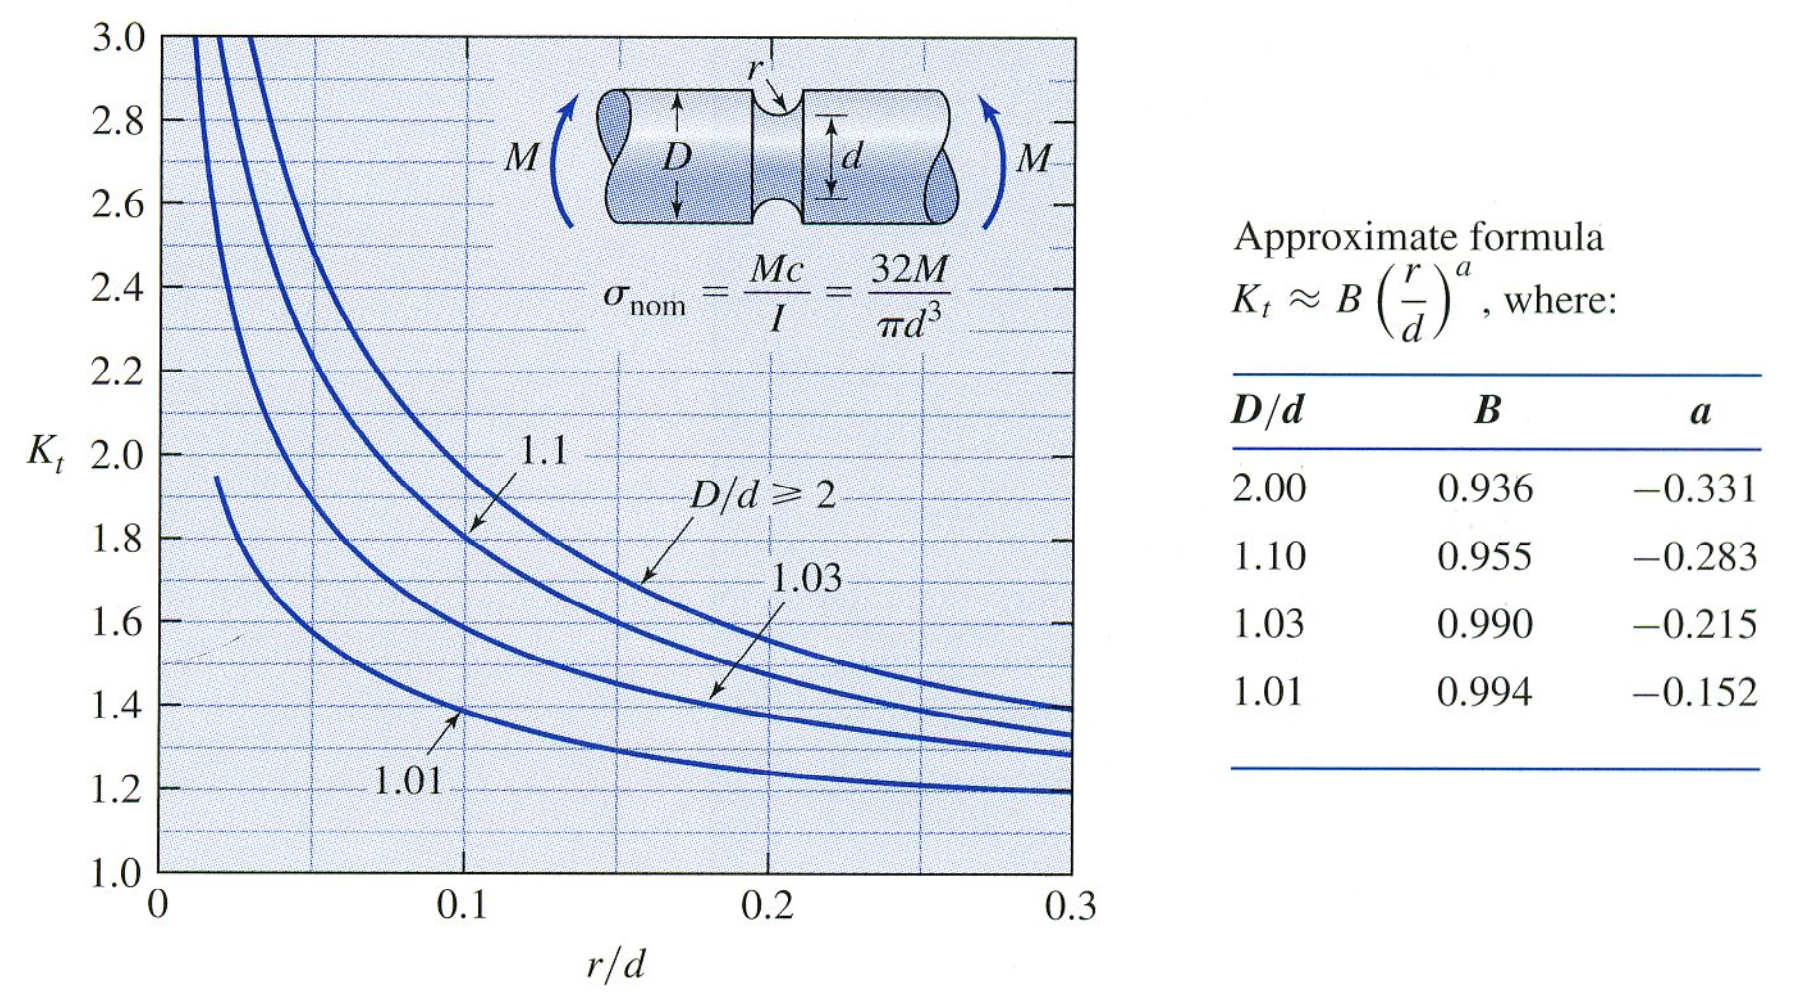
\includegraphics[width=0.45\textwidth]{05_design_factor/circlip-groove-bending.png}
    }
    \hfill{}
    \subfloat[Torsion]{
        \includestandalone[width=0.45\textwidth]{05_design_factor/circlip-groove-torsion}
        %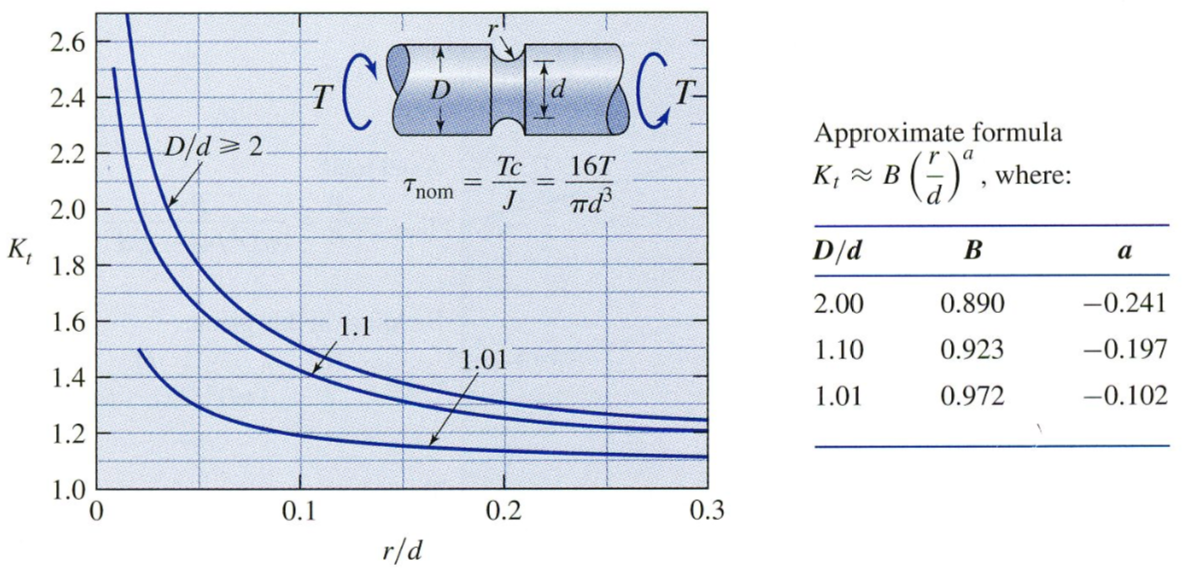
\includegraphics[width=0.45\textwidth]{05_design_factor/circlip-groove-torsion.png}
    }
    \hfill{}
    
    \vspace{1em}
    \caption{Circlip stress concentration factors for shafts}\label{fig-stress-circlip}
\end{figure*}

